% Copyright 2018-2024 Pietro Prandini
%
% This file is part of GuitarHub.
%
% GuitarHub is free software: you can redistribute it and/or modify
% it under the terms of the GNU General Public License as published by
% the Free Software Foundation, either version 3 of the License, or
% (at your option) any later version.
%
% GuitarHub is distributed in the hope that it will be useful,
% but WITHOUT ANY WARRANTY; without even the implied warranty of
% MERCHANTABILITY or FITNESS FOR A PARTICULAR PURPOSE.  See the
% GNU General Public License for more details.
%
% You should have received a copy of the GNU General Public License
% along with GuitarHub.  If not, see <https://www.gnu.org/licenses/>.

\vspace*{\stretch{3}}
\begin{center}
	{\textit{\textbf{This booklet is written by free (as in freedom) interpretations of the contributors.}}}\par
\end{center}
\vspace*{\stretch{2}}
\begin{center}
	\textbf{A special thanks to:}
	\begin{itemize}
	\item {\textit{\rmfamily Kevin Hamlen}}, author of the \href{http://songs.sourceforge.net/}{\textit{songs package}} and technical supporter, he has provided the package that is used by the project and he has given fast problems' solution;
	\item {\textit{\rmfamily Paweł Andrejczuk}}, english supporter, he has improved the english text;
	\item {\textit{\rmfamily Anna Libardi}}, licence consultant, she has given some useful informations;
	\item {\textit{\rmfamily Maria Zardini}}, ecological supporter, she has recycled the tests' paper;
  \item all the \href{https://github.com/PietroPrandini/GuitarHub/graphs/contributors}{other contributors}.
\end{itemize}

\end{center}
\vspace*{\stretch{2}}
\begin{center}
	{\textit{\footnotesize{A full list of the other contributors is available on \href{https://github.com/PietroPrandini/GuitarHub/graphs/contributors}{https://github.com/PietroPrandini/GuitarHub/graphs/contributors}}}}\par
%\medskip
%\qrcode[hyperlink,height=1.5cm]{https://github.com/PietroPrandini/GuitarHub/graphs/contributors}
\end{center}
\vspace*{\stretch{10}}
\begin{center}
	\href{http://creativecommons.org/licenses/by-sa/4.0/}{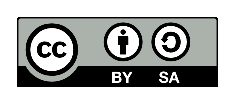
\includegraphics[scale=0.5]{img/cc-by-sa_88x31}} \par
	{\footnotesize{This work is licensed under the Creative Commons Attribution-ShareAlike 4.0 International License. To view a copy of this license, visit \href{http://creativecommons.org/licenses/by-sa/4.0/}{http://creativecommons.org/licenses/by-sa/4.0/} or send a letter to Creative Commons, PO Box 1866, Mountain View, CA 94042, USA.}}\par
\medskip
\qrcode[hyperlink,height=1.5cm]{http://creativecommons.org/licenses/by-sa/4.0/}
\end{center}
\vspace*{\stretch{1}}
\newpage
